\documentclass[headrule,footrule]{foils}

%%
%%%  Macros
%%%
%%% fonts-sil-charis for IPA in week 5

\newcommand{\logo}{HG2002 (2021)}
\usepackage[hidelinks]{hyperref}

\newcommand{\header}[3]{%
  \title{\vspace*{-2ex} \large 
    HG2002 Semantics and Pragmatics
% \thanks{Creative
%       Commons Attribution License: 
%       you are free to share and adapt as long as you give 
%       appropriate credit and add no additional restrictions: 
%       \protect\url{https://creativecommons.org/licenses/by/4.0/}.
%     }
    \\[2ex] \Large  \emp{#2} \\ \emp{#3}}
  \author{\blu{Francis Bond}   \\ 
    \normalsize  \textbf{Division of Linguistics and Multilingual Studies}\\
    \normalsize  \url{http://www3.ntu.edu.sg/home/fcbond/}\\
    \normalsize  \texttt{bond@ieee.org}}
  \MyLogo{\logo}
  % \MyLogo{奈良女子大学:欧米言語情報理論II}
  \date{#1
    \\  \url{https://bond-lab.github.io/Semantics-and-Pragmatics/}
\\[.5ex] \footnotesize Creative  Commons Attribution License:  you are free to share and adapt 
\\[-.25ex] \footnotesize   as long as you give    appropriate credit and add no
additional restrictions: 
\\ \small  \protect\url{https://creativecommons.org/licenses/by/4.0/}.
}
  % \renewcommand{\logo}{#2}
  % \special{! /pdfmark where
  %   {pop} {userdict /pdfmark /cleartomark load put} ifelse
  %   [ /Author (Francis Bond)
  %   /Title (#1: #2)
  %   /Subject (HG2002: Semantics and Pragmatics)
  %   /Keywords (Semantics, Pragmatics, Meaning)
  %   /DOCINFO pdfmark}
  %   }
  \hypersetup{%
    final       = true,
    colorlinks  = true,
    urlcolor    = blue,
    citecolor   = blue,
    linkcolor   = MidnightBlue,
    unicode     = true,
    pdfauthor   = {Francis Bond},
    pdfkeywords = {Semantics, Pragmatics, Meaning},
    pdftitle    = {#1: #2},
    pdfsubject  = {HG2002 Semantics and Pragmatics; License CC BY 4.0}
  }
}


\usepackage[a4paper,landscape]{geometry}
%\usepackage[dvips]{xcolor}
\usepackage[dvipsnames,x11names]{xcolor}
\usepackage{graphicx}
\newcommand{\blu}[1]{\textcolor{blue}{#1}}
\newcommand{\grn}[1]{\textcolor{green}{#1}}
\newcommand{\hide}[1]{\textcolor{white}{#1}}
\newcommand{\emp}[1]{\textcolor{red}{#1}}
\newcommand{\txx}[1]{\textbf{\textcolor{blue}{#1}}}
\newcommand{\lex}[1]{\textbf{\mtcitestyle{#1}}}


\usepackage{amsmath,latexsym}
\usepackage{pifont}
\renewcommand{\labelitemi}{\textcolor{violet}{\ding{227}}}
\renewcommand{\labelitemii}{\textcolor{purple}{\ding{226}}}

\newcommand{\subhead}[1]{\noindent\textbf{#1}\\[5mm]}

\newcommand{\Bad}{\emp{\raisebox{0.15ex}{\ensuremath{\mathbf{\otimes}}}}}
\newcommand{\bad}{*}

\newcommand{\com}[1]{\hfill \textnormal{(\emp{#1})}}%
\newcommand{\cxm}[1]{\hfill \textnormal{(\txx{#1})}}%
\newcommand{\cmm}[1]{\hfill \textnormal{(#1)}}%

\usepackage{relsize,xspace}
\newcommand{\into}{\ensuremath{\rightarrow}\xspace}
\newcommand{\ent}{\ensuremath{\Rightarrow}\xspace}
\newcommand{\nent}{\ensuremath{\not\Rightarrow}\xspace}
\newcommand{\tot}{\ensuremath{\leftrightarrow}\xspace}
\usepackage{url}
\newcommand{\lurl}[1]{\MyLogo{\url{#1}}}

\usepackage{mygb4e}
\let\eachwordone=\itshape
\newcommand{\lx}[1]{\textbf{\textit{#1}}}
\newcommand{\ix}{\ex\it}

\newcommand{\cen}[2]{\multicolumn{#1}{c}{#2}}
%\usepackage{times}
%\usepackage{nttfoilhead}
\newcommand{\myslide}[1]{\foilhead[-25mm]{\raisebox{12mm}[0mm]{\emp{#1}}}\MyLogo{\logo}}
\newcommand{\myslider}[1]{\rotatefoilhead[-25mm]{\raisebox{12mm}[0mm]{\emp{#1}}}}
%\newcommand{\myslider}[1]{\rotatefoilhead{\raisebox{-8mm}{\emp{#1}}}}

\newcommand{\section}[1]{\myslide{}{\begin{center}\Huge \emp{#1}\end{center}}}



\usepackage[lyons,j,e,k]{mtg2e}
\renewcommand{\mtcitestyle}[1]{\textcolor{teal}{\textsl{#1}}}
%\renewcommand{\mtcitestyle}[1]{\textsl{#1}}
\newcommand{\ja}[1]{\mtcitestyle{\makexeCJKactive #1\makexeCJKinactive}}
\newcommand{\chn}{\mtciteform}
\newcommand{\zsm}{\mtciteform}
%\newcommand{\cmn}[1]{make\cjkactive\mtciteform#1\makecjkinactive}
\newcommand{\iz}[1]{\textup{\texttt{\textcolor{blue}{\textbf{#1}}}}}
\newcommand{\con}[1]{\textsc{#1}}
\newcommand{\gm}{\textsc}
\newcommand{\cmp}[1]{{[\textsc{#1}]}}
\newcommand{\sr}[1]{\ensuremath{\langle}#1\ensuremath{\rangle}}
\usepackage[normalem]{ulem}
\newcommand{\ul}{\uline}
\newcommand{\ull}{\uuline}
\newcommand{\wl}{\uwave}
\newcommand{\vs}{\ensuremath{\Leftrightarrow}~}
%%% theta role
\newcommand{\tr}[1]{\textcolor{Chartreuse4}{\textsc{#1}}}
%%% theta grid
\newcommand{\grid}[1]{\ensuremath{\langle}\tr{#1}{\ensuremath{\rangle}}}

%%%
%%% Bibliography
%%%
\usepackage{natbib}
%\usepackage{url}
\usepackage{bibentry}
%\usepackage{CJKutf8}


\usepackage{fontenc}
\usepackage{polyglossia}
\setmainlanguage{english}
\setotherlanguages{tamil}
\setmainfont[Ligatures=TeX]{TeX Gyre Pagella}
\setsansfont[Ligatures=TeX]{TeX Gyre Heros}
\newfontfamily\ipafont{Charis SIL}
\newcommand\ipa[1]{\mtcitestyle{\ipafont #1}}


\usepackage{xeCJK}
\makexeCJKinactive
\newcommand{\zh}[1]{\mtcitestyle{\makexeCJKactive #1\makexeCJKinactive}}
%\newcommand{\ja}[1]{\makexeCJKactive #1\makexeCJKinactive}
\setCJKmainfont{Noto Sans CJK JP}
\setCJKsansfont{Noto Sans CJK SC}
\setCJKmonofont{Noto Sans CJK SC}

\newfontfamily\tamilfont[Script=Tamil]{Noto Sans Tamil}
\newfontfamily\tamilfontsf[Script=Tamil]{Noto Sans Tamil}
\newcommand{\tam}[1]{\texttamil{#1}}
%%% From Tim
\newcommand{\WMngram}[1][]{$n$-gram#1\xspace}
\newcommand{\infers}{$\rightarrow$\xspace}


\usepackage{rtrees,qtree}
\renewcommand{\lf}[1]{\br{#1}{}}
\usepackage{avm}
%\avmoptions{topleft,center}
\newcommand{\ft}[1]{\textsc{#1}}
\renewcommand{\val}[1]{\textit{#1}}
\newcommand{\typ}[1]{\textit{#1}}
\avmfont{\sc}
\avmvalfont{\sc}
\renewcommand{\avmtreefont}{\sc}
\avmsortfont{\it}


%%% From CSLI book
\newcommand{\mc}{\multicolumn}
\newcommand{\HD}{\textbf{H}\xspace}
\newcommand{\el}{\< \>}
\makeatother
\long\def\smalltree#1{\leavevmode{\def\\{\cr\noalign{\vskip12pt}}%
\def\mc##1##2{\multispan{##1}{\hfil##2\hfil}}%
\tabskip=1em%
\hbox{\vtop{\halign{&\hfil##\hfil\cr
#1\crcr}}}}}
\makeatletter

%\usepackage{tipa}
\usepackage{multicol}


\newcommand{\task}{\marginpar{\large ~~~\textbf{?}}}
\newcommand{\sh}[1]{\href{https://www.arthur-conan-doyle.com/index.php?title=#1}{#1}}

\usepackage{tikz}
\usepackage{tikz-qtree}
\usepackage{forest}




\begin{document}
\header{Lecture 2}{Meaning, Thought and Reality}{}\maketitle

%\include{schedule}

\myslide{Overview}

\begin{itemize}
\item Revision
  \begin{itemize}
  \item Introduction to Semantics
  \item Information Theory
  \end{itemize}
\item Reference
\item Reference as a Theory of Meaning
\item Mental Representations
\item Deixis
\item Words, Concepts and Thinking
\end{itemize}
\begin{center}
  A lot of material will be covered, we will revisit most of it
\end{center}

%%%
%%% this changes each year, so keep separate
%%%
\include{schedule}

% \myslide{Administrivia}
% \begin{description}\addtolength{\itemsep}{-5mm}
% \item [Coordinator]  Francis \ul{Bond} 
% {\small \url{<bond@ieee.org>} !\url{<fcbond@ntu.edu.sg>}}
% \item [Tutor]  Joanna \ul{Sio} Ut Seong 
% {\small \url{<neosome@gmail.com>} !\url{<ussio@ntu.edu.sg>}}
% \item [Lecture] Tuesday 9:30--11:30 (SPMS-LT3)
% \item [Tutorials] Tuesday 
%   \begin{itemize}
%   \item 11:30--12:30 (T1: SPMS-TR+19 \textbf{FB}; T2: SPMS-TR+20 \textbf{JS})
%   \item 12:30--13:30 (T3: TR+19 \textbf{JS}); 14:30--15:30 (T3: TR+19 \textbf{JS});
%   \end{itemize}
%  T1 (17+2); T2 (20+4); T3 (19+1); T4 (0)
% \item[Office hours] ~
%   \begin{tabular}[t]{llr}
% Francis & Tuesday &  14:00--15:00   \\  
% Francis & Thursday &  10:00--11:00   \\
% Joanna  & Friday & 9:30--11:30 
%   \end{tabular}
% \end{description}

\section{Revision: \\ Introduction to Semantics}

\myslide{What is Semantics}
\begin{itemize}
\item Very broadly, semantics is the study of meaning
  \begin{itemize}
  \item Word meaning
  \item Sentence meaning
  \end{itemize}
\item Layers of Linguistic Analysis
  \begin{enumerate}%\addtolength{\itemsep}{-0.75ex}
  \item Phonetics \& Phonology
  \item Morphology
  \item Syntax
  \item \emp{Semantics}
  \item Pragmatics
  \end{enumerate}
\item Semantics could be \txx{autonomous} or \txx{integrated} with other knowledge
\end{itemize}

\myslide{Meaning in the larger context}

\begin{itemize}
\item \txx{Semiotics} is the study of interpreting symbols, or \txx{signification}
  \begin{itemize}
  \item We refer to the \txx{signified}
  \item Using a \txx{signifier}\hfill Saussure
  \end{itemize}
\item Problems with defining meaning
  \begin{itemize}
  \item The \txx{grounding} problem and \txx{circularity}
  \item The boundaries of meaning: \txx{linguistic} vs \txx{encyclopedic knowledge}
  \item Individual variation in meaning: \txx{idiolects}
  \item Words can be combined to form an infinite number of expressions
    \begin{itemize}
    \item This building up of meaning is referred to as \txx{composition}
    \item If the meaning of the whole can be built up from the parts then it is \txx{compositional}
  \end{itemize}
\end{itemize}
\end{itemize}

\myslide{Metalanguages and Notational Conventions}

We use language to talk about language, which can get messy.  So we
try to use certain words with very specific technical senses.

\begin{itemize}
\item \txx{technical term} $\leftarrow$ remember me!
\item \eng[gloss]{word} or \eng{utterance}
\item \lex{lexeme}
\item \iz{predicate}
\item \con{concept}
\end{itemize}
\myslide{Utterances, Sentences and Propositions}

\begin{itemize}
\item \txx{utterance}: an actual instance of saying (or writing  or \ldots) something
\item \txx{sentence}: an abstraction, the type of what was said
  \begin{exe}
    \ex \eng{Caesar invades Gaul}
  \end{exe}
\item \txx{proposition}: a further abstraction, normally ignoring some non-literal meaning
  \begin{exe}
    \ex \iz{invade(Caesar, Gaul)}
  \end{exe}
  \begin{itemize}
  \item \txx{information structure}: what part of a proposition is emphasized
 \begin{exe}
   \ex \eng{Caesar invaded Gaul}
   \ex \eng{Gaul was invaded by Caesar}
   \ex \eng{It was Gaul that  Caesar invaded}
   \ex \eng{It was Caesar who invaded Gaul}
  \end{exe}
  \end{itemize}

\end{itemize}

\myslide{Information Theory}
\MyLogo{not in Saeed}
\begin{itemize}
\item Language has many uses, only one of which is to convey information
%  \\ \textit{A bit of Fry and Laurie Season 1 Episode 2}
  \\ --- but surely transferring information is important
\item We can measure information in a limited, technical, and very useful, sense
  \begin{itemize}
  \item Think of a \txx{signal} being transmitted from a source to a
    destination, possibly with \txx{noise} in the channel
  \item Measure Information in \txx{bits}: 
    \\ the number of yes/no questions needed to determine a term
  \item Context can help decoding due to \txx{Mutual Information}
  \end{itemize}
\newpage 
\item How can we get our message across efficiently and safely?
  \begin{itemize}
  \item \txx{Optimal encoding} can make the transmission efficient
    \\ Frequent expressions should be short
  \item \txx{Redundant encoding} can make the transmission robust
  \end{itemize}
\end{itemize}

\section{Meaning, Thought and Reality}
\MyLogo{}


\myslide{Referential or Representational?}

\begin{exe}
  \ex \eng{I kicked the dog.}
  \ex \eng{I did not kick the dog.}
\end{exe}

Assuming that they were uttered at the same time, they are
incompatible because they cannot refer to the same
situation. 

But we can represent the same reality in different ways:

\begin{exe}
  \ex \eng{Ich habe Hunger} ``I have hunger''
  \ex \eng{I am hungry}
\end{exe}

Representational theories are interested in how we represent reality,
and how our representations are influenced by conceptual structures
conventionalized in language.


 \myslide{Referential View}

 \begin{center}
   \setlength{\unitlength}{2mm}
   \begin{picture}(80,50)(0,0) \put(5,35){\oval(25,6)}
     \put(5,35){\makebox(0,0){\bf Speaker}}

     \put(25,25){\oval(25,6)}
     \put(25,25){\makebox(0,0){\bf Expression}} 

     \put(75,25){\oval(25,6)}
     \put(75,25){\makebox(0,0){\bf Referent}} 

     \put(37.5,25){\vector(1,0){25}}
     \put(50,20){\makebox(0,0){Denote}}

     \put(17.5,35){\vector(1,-0.15){45}}
     \put(50,35){\makebox(0,0){Refer}}

     \put(5,32){\vector(1,-0.20){17}}
     \put(3,30){\makebox(0,0){Say}}

   \end{picture}
 \end{center}

 \txx{Referential view}  is focused on direct relationships between expressions (words, sentences) and things in the world (realist view).  
\\(More in Chapter 10: Formal Semantics)




 \myslide{Representational View}

 \begin{center}
   \setlength{\unitlength}{2mm}
   \begin{picture}(80,50)(0,0) \put(5,35){\oval(25,6)}
     \put(5,35){\makebox(0,0){\bf Speaker}}

     \put(25,25){\oval(25,6)}
     \put(25,25){\makebox(0,0){\bf Expression}} 

     \put(50,40){\oval(25,6)}
     \put(50,40){\makebox(0,0){\bf Concept}} 

     \put(75,25){\oval(25,6)}
     \put(75,25){\makebox(0,0){\bf Referent}} 


     % \put(37.5,25){\vector(1,0){25}}
     % \put(50,20){\makebox(0,0){Experience}}

     \put(25,28){\vector(1,0.35){26}}
     \put(30,33){\makebox(0,0){Denote}}

     \put(17.5,35){\vector(1,0.2){20}}
     \put(30,40){\makebox(0,0){Refer}}

     \put(5,32){\vector(1,-0.20){17}}
     \put(3,30){\makebox(0,0){Say}}

     \put(50,37){\vector(1,-0.35){26}}
     \put(75,33){\makebox(0,0){Represent}}
   \end{picture}
 \end{center}
\vspace{-4em} \txx{Representational view} is focused on how relationships between
 expressions (words, sentences) and things in the world are mediated by
 the mind (cognitive linguistics).  
\\(More in Chapters 9 and 11: Meaning Components and Cognitive Linguistics)


\myslide{Referring vs Non-Referring}

\begin{itemize}
\item \txx{Referring expressions} are expressions that identify
  entities in the world (typically \txx{nominals})
  \begin{exe}
    \ex \eng{cat}, \jpn[that yellow bag]{ano kiiro kaban}
    \ex \eng{London Bridge}, \eng{Xiao Ming}
  \end{exe}
\item \txx{Non-referring expressions} don’t have referential properties
  \begin{exe}
    \ex \eng{maybe, if, is, but}
  \end{exe}
\item Not all nominals refer
  \begin{exe}
    \ex \eng{That is \ul{an ugly dog}}
    \ex \eng{If only I had \ul{a dog}}
  \end{exe} 
\end{itemize}

\myslide{Constant vs Variable Reference}
\begin{itemize}
\item Expressions with \txx{constant reference} are independent of context of utterance
  \begin{exe}
    \ex \eng{Ang Mo Kio, Great Wall of China, NTU Provost}
  \end{exe}
  Although possibly time dependent.  
\\ And what about models?
\item Expressions with \txx{variable reference} are dependent on the
  context of utterance (\txx{deixis} Ch 7)
  \begin{exe}
    \ex  \eng{I, you, he, she, them}
  \end{exe}
\end{itemize}
\myslide{What does it mean to know Shakespeare?}

\myslide{The description theory (Frege/Russell/Searle)}

Names are like abbreviations for descriptions:

\begin{quote}
  \eng{William Shakespeare} = ``the playwright who wrote Hamlet''  
\end{quote}


\begin{itemize}
\item They give the necessary conditions to identify someone
\item This emphasises that to know the referent of a name, you have to have
some knowledge of that referent.
\item understanding a name and identifying a referent are dependent on associating the name with the right description
\end{itemize}

\myslide{The causal theory (Kripke)}

Names begin with some event of naming (e.g. a christening) before
becoming commonly accepted.  They are just labels.

\begin{quote}
  \eng{William Shakespeare} = ``the guy other people call William Shakespeare''  
\end{quote}
\begin{itemize}
\item This emphasises that to know the meaning of a name is the result
  of this original event or grounding of the name.
\item The name itself doesn’t really ``mean'' anything- it ``points''
  to an individual.
\item It explains somewhat why names are arbitrary
\end{itemize}

\myslide{Nominal Reference}

\begin{exe}
  \ex \eng{I read \ul{a book} \cxm{indefinite}}
  \ex \eng{I read \ul{a book about semantics}}
  \ex \eng{I read \ul{the book} \cxm{definite}}
  \ex \eng{I read \ul{the book recommended by Lyons}} 
  \ex \eng{The \ul{king of France} is bald} 
  \begin{xlist}
    \ex \eng{There is a \ul{king of France}} \cxm{presupposition}
  \end{xlist}
  \ex \eng{\ul{The students} mistrusted each other} \cxm{distributive}
  \ex \eng{\ul{The students} couldn't fit into the lift} \cxm{collective}
  \ex \eng{\ul{Every student} enjoyed the lecture} \cxm{quantification}
  \ex \eng{\ul{All students} enjoyed the lecture} \cxm{quantification}
  \ex \eng{\ul{No students} enjoyed the lecture}\cxm{quantification}
  \ex \eng{\ul{Every student} didn't enjoy the lecture, it was really dull}\cxm{quant.}
  \ex \eng{\ul{Every student} didn't enjoy the lecture, but most did}\cxm{quant.}
\end{exe}

\myslide{Reference as a Theory of Meaning}

\begin{itemize}
\item Meaning as denotation (the link between expression and the world)\\ 
  \begin{tabular}{lll}
    names & denote & individuals \\   
    common nouns & denote & sets of entities \\
    verbs  & denote & actions \\    
    adjectives  & denote & properties of entities \\
    adverbs  & denote & properties of actions \\
  \end{tabular}
\item Doesn't account for \eng{no, some, up, if}
\item What about things that don't exist?
  \begin{exe}
    \ex \eng{I like paintings of \ul{unicorns}}
  \end{exe}
\item What about different descriptions of the same referent?
  \begin{exe}
    \ex \eng{\ul{Soylent Green} is \ul{people}}
  \end{exe}
\end{itemize}

\myslide{Mental Representations}

\begin{itemize}
\item Divide meaning into
  \begin{itemize}
  \item \txx{reference}: the relation to the world
  \item \txx{sense}: the rest of the meaning
  \end{itemize}
\item Introduce \txx{concepts} \hfill (meaning as font-change)
  \begin{itemize}
  \item How can we represent concepts?
  \item How do we learn them?
    \begin{itemize}
    \item Typically children start off by \txx{underextending} or \txx{overextending} concepts
    \end{itemize}
  \end{itemize}
\end{itemize}

\myslide{Necessary and Sufficient Conditions}

\begin{itemize}
\item Can we define words in terms of \txx{conditions}?
  \begin{itemize}
  \item \lex{zebra}
    \begin{itemize}
    \item quadruped
    \item animal \com{redundant}
    \item black and white striped
    \item herbivore
    \end{itemize}
  \end{itemize}
\item These are \txx{generic} properties
\item Can we use words even if we don't know their properties?
  \begin{itemize}
  \item \lex{Kway Teow}
  \end{itemize}
\item We seem to have fairly vague definitions
\end{itemize}

\myslide{Video: The Blackberry Sketch}
\MyLogo{The One Ronnie}

\begin{itemize}
\item Define the following:
  \begin{itemize}
  \item \lex{blackberry}
  \item \lex{orange}
  \item \lex{apple}
  \item \lex{date}
  \end{itemize}
\item How similar are your definitions to the use in the video?
\end{itemize}



\section{Deixis}


\myslide{What is Deixis}
\begin{itemize}
\item any linguistic element whose interpretation
  necessarily makes reference to properties of the
  extra-linguistic context in which they occur is \txx{deictic}
  \begin{description}
  \item[\txx{Person}] relative to the speaker and addressee; \eng{you, me, them}
  \item[\txx{Spatial Location}] demonstratives; \eng{this, that, over there, here}
  \item[\txx{Temporal Location}] tense; \eng{yesterday, today, tomorrow}
  \item[\txx{Social Status}] relative to the social position: \eng{professor, you, uncle, boy}
  \end{description}
\item \txx{Discourse deixis}: referring to a linguistic expression or chunk of discourse
\end{itemize}

More than 90\% of the declarative sentences people utter are indexical
in that they involve implicit references to the speaker, addressee,
time and/or place of utterance in expressions like first and second
person pronouns, demonstratives, tenses, and adverbs like \lex{here}, \lex{now},
\lex{yesterday} \citep[p366]{Bar-Hillel:1954}.

\myslide{Spatial Deixis}

\begin{itemize}
\item Two (three) way systems (English, \ldots)
  \\[2ex] \begin{tabular}{llll}
    \txx{proximal} &\lex{this} & \lex{here} &close to the speaker\\
    \txx{distal} &\lex{that} & \lex{there} & far to the speaker \\[1ex]
    \txx{Q} &\lex{what} & \lex{where} & unknown
  \end{tabular}
\item Three (four) way systems (Japanese, \ldots)
    \\[2ex] \begin{tabular}{llll}
      \txx{proximal}& \lex{kore} ``this'' & \lex{koko} ``here'' & close to speaker\\
      \txx{medial} &\lex{sore} ``that''   & \lex{soko} ``there'' &close to addressee\\
      \txx{distal} &\lex{are} ``that'' & \lex{asoko} ``over there''
                                                                &far
                                                                  from
                                                                  both
              \\[1ex]  % \hline
      \txx{Q} &\lex{dore} ``what'' & \lex{doko} ``where'' & unknown 
  \end{tabular}
  \item Can decompose: \lex{here} ``this place'', \lex{there} ``that place'', \lex{where} ``what place''
 \lex{now} ``this time'',  \lex{then} ``that time'', \lex{when} ``what time''
\end{itemize}

% \myslide{More complicated deictic systems exist}

% Qiang directional prefixes (LaPolla 2003: 581)

% \begin{tabular}{llll}
% 	\lex{t\textschwa{}l}& 'look upward'& \lex{\texthth\textscripta{}l}& 'look downward'\\
% 	\lex{z\textschwa{}l}& 'look toward centre'& \lex{d\textscripta{}l}& 'look outward from centre'\\
% 	\lex{h\textschwa{}l}& 'look upstream'& \lex{s\textschwa{}l}& 'look downstream'\\
% 	\lex{\textschwa{}l}& 'look in'& \lex{h\textscripta{}l}& 'look out'
%       \end{tabular}

\myslide{More complicated still}
  
 Mongsen Ao directional motion verbs (Coupe 2007: 280-282)

 \begin{tabular}{llll}
   A& \lex{k\textschwa{}wa}& (ascend+go.pst)& ‘went up’\\
   B& \lex{k\textschwa{}\textturnr{}a}& (ascend +come.pst)& ‘came up’\\
   C& \lex{hl\`a} & (descend+go.pst)& ‘went down’\\
   D& \lex{l\textschwa{}\textturnr{}a~lala}& (descend+come.pst)& ‘came down’\\
   E& \lex{hja}& (level+go.pst)& ‘went across’ (same level)\\
   F& \lex{hi\textturnr{}a}& (level+come.pst)& ‘came across’ (same level)\\
 \end{tabular}

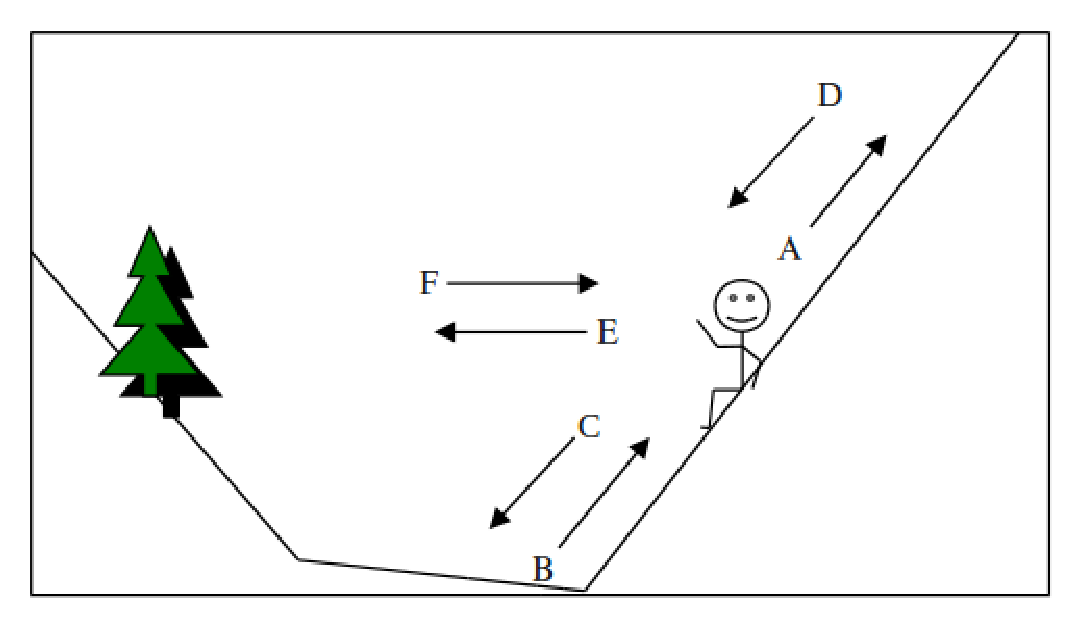
\includegraphics[height=0.4\textheight]{pics/Mongsen-ao}


\myslide{More Spatial Deixis}

\begin{itemize}
\item Often lexicalized:
  \begin{itemize}
  \item \lex{go, come, foreign, home, local, indigenous, national language}
  \end{itemize}
\item Can lead to \txx{discourse}/\txx{textual deixis}
  \begin{exe}
    \ex \eng{\ul{Here} we begin explaining textual deixis}
  \end{exe}
\item Often also used for time
  \begin{exe}
    \ex \eng{\ul{This year} we are trying a new kind of assignment}
  \end{exe}
\newpage
\item Spatial expressions often extend to possession
  \begin{exe}
    \ex \gll \jpn{NICT-ga} \jpn{Kyoto-ni} \jpn{aru} \\
    NICT-\textsc{nom} Kyoto-\textsc{loc} be \\
    \trans NICT is in Kyoto
    \ex \gll \jpn{watashi-ni} \jpn{musuko-ga}  \jpn{aru} \\
     I-\textsc{loc}  son-\textsc{nom} be \\
    \trans I have a son (lit. a son is in me)
   \end{exe}
\end{itemize}

\myslide{Person Deixis}

\begin{itemize}
\item Minimally a three way division
\\[2ex]  \begin{tabular}{lll}
    First Person & Speaker & \lex{I} \\
    Second Person & Addressee & \lex{you} \\
    Third Person & Other & \lex{he/she/it} \\
  \end{tabular}
\item Often combined with
  \begin{itemize}
  \item \txx{gender}: \lex{he/she/it }
  \item \txx{number}: \lex{I/we}, 
    \lex{'anta} ``you:m'', \lex{'antumaa} ``you:dual'',  \lex{'antum} ``you:m:pl''
    \\ (Arabic)
  \item \txx{inclusion}: \lex{n\'uy} ``we including you'',  \lex{n\'{\i}i} ``we excluding you'' (Zayse)
  \item \txx{honorification}: \lex{kimi} ``you:inferior'', \lex{anata} ``you:equal'',
    \\ don't use pronouns for superiors: \lex{sensei} ``teacher'', \ldots (Japanese)
  \end{itemize}
\end{itemize}

\myslide{Social Deixis}

In European languages, a two-way choice in 2nd person pronominal
reference is known as the T/V distinction, based on the French forms
for ``you''.

\begin{itemize}
\item T/V distinctions in European languages
\\[2ex]  \begin{tabular}{lll}
    & Familiar 2sg & Polite 2sg \\ \hline
    French & tu & vous \\
    German & du & Sie \\
    Spanish & t\'u & usted
  \end{tabular}

\item Shift from asymmetric use showing \txx{power} (superior uses \lex{du}; inferior uses \lex{vous}) to symmetric use showing \txx{solidarity} (strangers use  \lex{vous}; intimates use \lex{du}): typically the socially superior person must invite the socially
  inferior person to use the familiar form
\end{itemize}

\myslide{Social Deixis can be marked on other words}
\MyLogo{It must be marked}
\begin{exe}
  \ex \jpn{Tanaka-san-ga kudasaimashita} \hfill [addressee and subject hon.]
  \trans Tanaka gave it to me
%  \trans
 \ex \jpn{Tanaka-san-ga kudasatta} \hfill [subject honorification]
  \trans Tanaka gave it to me

 \ex \jpn{Tanaka-kun-ga kuremashita} \hfill [addressee honorification]
  \trans Tanaka gave it to me

 \ex \jpn{Tanaka-kun-ga kureta} \hfill [no honorification]
  \trans Tanaka gave it to me

\end{exe}

\myslide{Types of Deixis}
\MyLogo{}
(a) Gestural; (b) Symbolic: (c) Non-deictic uses (Levinson 1983:66):
\begin{exe}
\ex \begin{xlist}
\ex \eng{You, you, but not you, are dismissed}
\ex \eng{What did you say?}
\ex \eng{You can never tell what they want  nowadays}
\end{xlist}
\ex \begin{xlist} 
\ex \eng{This finger hurts}
\ex \eng{This city stinks}
\ex \eng{I met this weird guy the other day}
\end{xlist}
\ex \begin{xlist} 
\ex \eng{Push, not now, but now}
\ex \eng{Let’s go now rather than tomorrow}
\ex \eng{Now, that is not what I said}
\end{xlist}
\ex \begin{xlist} 
\ex \eng{Not that one, idiot, that one}
\ex \eng{That’s a beautiful view}
\ex \eng{Oh, I did this and that}
\end{xlist}
% \ex \begin{xlist}
% \ex \eng{Move it from there to there
% \ex \eng{Hello, is Harry there?
% \ex \eng{There we go
% \end{xlist}  
\end{exe}




\myslide{Non-standard usage of deixis}

\begin{exe}
  \ex \eng{You take your screwdriver, right, and screw her home}
  \ex \eng{Are we ready for our medicine now, Dr Smith? }
  \ex \eng{We now turn to a discussion of globalisation in Chapter Three}
  \ex \eng{When you’re hot you’re hot}
  \ex \eng{Sometimes you wonder about the quality of the political leadership}
  \ex \eng{She's a beauty all right} \textnormal{[said of a car]}
\end{exe}



% \myslide{Anaphora}
% \begin{itemize}
% \item Referring to some referent described elsewhere in the discourse
% \begin{itemize}
%   \item Nominal: \eng{it, the animal}
%   \item Temporal: \eng{then} 
%   \item Backward (cataphora): if the referent comes after.
%   \end{itemize}
% \item Anaphoric elements
%   \begin{itemize}
%   \item are semantically underspecified, thus are referentially dependent upon their
%     antecedents
%   \item play an important referent tracking role in discourse, because they encode
%     topic continuity
%   \end{itemize}
% \end{itemize}


\myslide{Strict and Sloppy Readings}
\MyLogo{Today's joke}
\begin{exe}
  \ex Wife: \eng{Jim kisses \ul{his wife} goodbye before he leaves for work every morning. Why don’t you do that?}
  \ex Husband: \eng{I don't know \ul{her} that well.}
\end{exe}
\begin{itemize}
\item \txx{Sloppy anaphora}  is the wife’s intended
  reading, where \eng{do that} is understood as ``kiss one's wife'',
  resolving to ``kiss your (own) wife''.
\item \txx{Strict anaphora} is the funny reading, where \eng{do that}
  is understood as ``kiss Jim’s wife''
\end{itemize}


\section{Concepts}

\myslide{Prototypes}

\begin{itemize}
\item Concepts are organized in groups around a \txx{prototype}
\item These have typical members (remembered as \txx{exemplars}) 
  \begin{itemize}
  \item What is typical \con{furniture}?
  \item What is a typical \con{bird}?
  \end{itemize}
\item prototypes have \txx{characteristic feature}s
  \begin{itemize}
  \item has feathers
  \item warbles
  \item flies
  \item lays eggs
  \end{itemize}
\item This work was pioneered by Eleanor Rosch (1973, 1975) (very readable)
\end{itemize}

% \myslide{What is a protoypical bird?}

% \\includegraphics[width=\textwidth]{pics/prot

\myslide{Relations between Concepts}

\begin{itemize}
\item Concepts are linked in many ways
\item Most common relationship is \txx{hypernymy}: \con{dog} is-a \con{animal}
\item Typically subordinate terms inherit from superordinate terms
\item Larger units of knowledge, such as \txx{frames} are similar
\item Much recent computational work on these
  \begin{itemize}
  \item WordNet
  \item FrameNet
  \end{itemize}
\end{itemize}



\myslide{Basic Level Categories}
\begin{itemize}
\item Some categories (concepts) seem to be more psychologically basic than others
  \begin{itemize}
  \item Pictures of objects are categorized faster at the basic level
  \item Basic level names used more often in free-naming tasks
  \item Children learn them earlier
  \item Basic-level names are more common in adult discourse 
  \item Basic-level categories are common in different cultures
  \item Basic level names tend to be short
  \item Basic-level names tend to be common in compound nouns
  \end{itemize}
\item
  \begin{tabular}[t]{lll}
superordinate & basic & subordinate \\  \hline
\lex{vehicle} & \lex{bus} & \lex{school bus} \\
\lex{jewelry} & \lex{necklace} & \lex{pearl necklace} \\
\lex{animal} & \lex{dog} & \lex{poodle} 
\end{tabular}
\end{itemize}

\myslide{}
\begin{itemize}
\item Basic level categories are a decomposition of the world into
  maximally informative categories. 
  \begin{itemize}
  \item BLCs maximize the number of attributes shared by members of
    the category
  \item BLCs minimize the number of attributes shared with
    other categories
  \end{itemize}
\item It can be hard to agree on what is the Basic Level: whereas dog
  as a basic category is a species, bird or fish are at a higher
  level, etc.
\item Similarly, the notion of frequency is very closely tied
  to the basic level, but not exactly the same.
\end{itemize}

\myslide{Linguistic Relativity}

\begin{itemize}
\item The language we think in makes some concepts easy to express,
  and some concepts hard
\item The idea behind \txx{linguistic relativity} is that this will
  effect how you think
  \begin{itemize}
  \item Korean lexicalizes politeness and has rigid social hierarchies
  \item English and Chinese speakers differ as to whether they
    concepualize things as substances or individuals
  \item Gendered language speakers have different connotations: \lex{key}
    \begin{itemize}
    \item (German: masculine) `hard, heavy, jagged, metal, and useful'
    \item (Spanish: feminine)  `golden, intricate, little, lovely, shiny, and tiny'
    \end{itemize}
  \item It is easier to differentiate colors that you have names for
  \end{itemize}
\item Most confirmed differences are very, very subtle
\end{itemize}


\myslide{The Sapir-Whorf Hypothesis}

\begin{description}
\item[strong]  language determines thought and that linguistic categories limit and determine cognitive categories
\item[weak]  linguistic categories and usage influence thought and certain kinds of non-linguistic behaviour
\end{description}

The terms "Strong/Weak Sapir-Whorf Hypothesis" is widely used even though Edward
Sapir and Benjamin Lee Whorf never co-authored anything and never
stated their ideas in terms of a hypothesis let alone with two versions.

\myslide{What Whorf actually said}
\begin{quotation}
  We dissect nature along lines laid down by our native language. The
  categories and types that we isolate from the world of phenomena we
  do not find there because they stare every observer in the face; on
  the contrary, the world is presented in a kaleidoscope flux of
  impressions which has to be organized by our minds—and this means
  largely by the linguistic systems of our minds. We cut nature up,
  organize it into concepts, and ascribe significances as we do,
  largely because we are parties to an agreement to organize it in
  this way—an agreement that holds throughout our speech community and
  is codified in the patterns of our language [\ldots] all observers
  are not led by the same physical evidence to the same picture of the
  universe, unless their linguistic backgrounds are similar, or can in
  some way be calibrated.
\\ \hfill Whorf (Carroll; Ed.); 1956: pp. 212–214
\end{quotation}


\myslide{Language, Thought and Reality}

\begin{itemize}\addtolength{\itemsep}{-1ex}
\item Do we really think in language? 
  \begin{itemize}
  \item We can think of things we don't have words for
  \item Language under-specifies meaning
  \end{itemize}
\item Maybe we store a more abstract representation
\\ \txx{the language of thought} or \txx{Mentalese}
\item Does the world exist outside of our minds?
\item If so, can we truly perceive it?
\item Many linguists side-step these issues: \txx{lexical semantics}
\item Many simplify them: \txx{formal semantics}
\item Some meet them head on: \txx{conceptual/cognitive semantics}
\end{itemize}

\myslide{Summary}
\begin{itemize}
\item Revision
  \begin{itemize}
  \item Introduction to Semantics
  \item Information Theory
  \end{itemize}
\item Reference
\item Reference as a Theory of Meaning
\item Mental Representations
\item Words, Concepts and Thinking
\end{itemize}


\emp{Next Week} Chapter 3: Word Meaning


\myslide{Acknowledgments and References}
\MyLogo{}
\begin{itemize}
\item Course design and slides borrow heavily from Nala Lee's course (HG202).
\item More about names and naming in: \\
Cumming, Sam, "Names", \textit{The Stanford Encyclopedia of Philosophy (Spring 2012 Edition),} Edward N. Zalta (ed.), 
URL = \url{<http://plato.stanford.edu/archives/spr2012/entries/names/>.} 
\item Video: Ronnie Corbet (2010) ``Blackberry Sketch'' In \textit{The One Ronnie}
broadcast on the BBC, 2012-12-17 
\item A great paper about doing research (no relation at all to semantics):
\\
\textit{You and your Research}  Richard Hamming
\\ Transcription of the Bell Communications Research Colloquium Seminar, 7 March 1986 
\\ \url{http://www.cs.virginia.edu/~robins/YouAndYourResearch.html}
\item Strict/sloppy identity joke adapted from \textit{Literal-Minded Blog:
Linguistic commentary from a guy who takes things too literally}.
\\ \footnotesize\url{http://literalminded.wordpress.com/2011/03/04/you-cant-go-from-strict-to-sloppy/}


\end{itemize}

\small
\bibliographystyle{aclnat}
\bibliography{abb,mtg,nlp,ling}

\end{document}
%%% Local Variables: 
%%% coding: utf-8
%%% mode: latex
%%% TeX-PDF-mode: t
%%% TeX-engine: xetex
%%% End: 

